\documentclass[a4paper]{article}
\usepackage[utf8]{inputenc}
\usepackage{fullpage}
\usepackage{csquotes}
\usepackage[ngerman]{babel}
\usepackage{biblatex}
\usepackage{float}
\usepackage{graphicx}
\usepackage{subfigure}
\usepackage[table]{xcolor}
\usepackage[format=plain,labelfont=bf,up]{caption}
\setcounter{secnumdepth}{-1} 
\usepackage{hyperref}
\usepackage{minted}
\usemintedstyle{friendly}
\bibliography{bibliography}
\title{Tenzing \\ A SQL Implementation On The MapReduce Framework}
\author{Willi Schönborn}
\date{\today}
\begin{document}

\begin{figure}[H]
\centering

\includegraphics[width=0.5\textwidth]{beuth.eps}
\maketitle
\end{figure}

\newpage

\tableofcontents

\newpage

\section{Einleitung}
Als Teil der Lehrveranstaltung \textit{Programmierung - Fortgeschrittene Konzepte} im Wintersemester 2011/2012 an der \textit{Beuth Hochschule für Technik Berlin} sollte im Rahmen einer Semesterarbeit ein wissenschaftliches Paper ausgewählt, untersucht und bewertet werden. Das Ziel dieses Dokumentes ist es die Ergebnisse dieser Semesterarbeit zusammenzufassen.

Ausgewählt wurde das Google-Paper \textit{Tenzing A SQL Implementation On The MapReduce Framework} \cite{TENZING}. Erschienen ist das Paper als Teil der Proceedings zur 37th VLDB, der \textit{International Conference on Very Large Data Bases} im September 2011. Die Autoren sind die Google-Mitarbeiter Biswapesh Chattopadhyay, Liang Lin, Weiran Liu, Sagar Mittal, Prathyusha Aragonda, Vera Lychagina, Younghee Kwon und Michael Wong.

\section{Kurzbeschreibung}
Tenzing beschreibt eine SQL92-kompatible Implementierung auf Basis des Google-eigenen MapReduce-Frameworks \cite{MAPREDUCE}.

\newpage

\section{MapReduce}

\subsection{Definition}

\begin{quote}
MapReduce is a programming model and an associated implementation for processing and generating large data sets. \cite{MAPREDUCE}
\end{quote}

\begin{quote}
MapReduce is a software framework introduced by Google in 2004 to support distributed computing on large data sets on clusters of computers. \cite{WP-MAPREDUCE}
\end{quote}

\begin{quote}
Hadoop MapReduce is a software framework for easily writing applications which process vast amounts of data (multi-terabyte data-sets) in-parallel on large clusters (thousands of nodes) of commodity hardware in a reliable, fault-tolerant manner. \cite{HADOOP}
\end{quote}

\subsection{Motivation}

\subsection{Funktionsweise}

\begin{figure}[H]
\centering
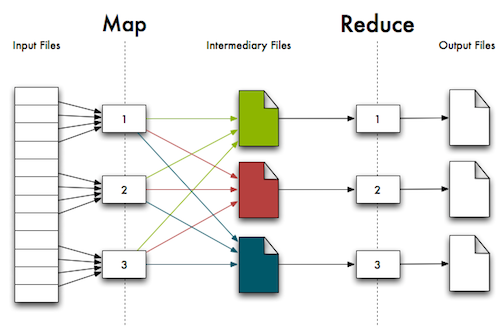
\includegraphics[width=0.8\textwidth]{mapreduce.png}
\caption{Die zwei Phasen eines MapReduce-Jobs \protect\cite{GARFINKEL}}
\end{figure}

\subsection{Open Source}
Googles Implementierung des MapReduce-Frameworks ist nicht öffentlich verfügbar. Die Apache Software Foundation hat sich mit dem Hadoop-Projekt zum Ziel gesetzt ein freies MapReduce-Ecosystem zu entwickeln.

\newpage

\section{SQL}
SQL steht für \textit{Structured Query Language} und ist eine mengenorientierte, deklarative Abfragesprache für Datenbank-Management-Systeme.

DML
DDL

\subsection{Syntax und Sprachelemente}

\begin{listing}[H]
\begin{minted}{sql}
SELECT [DISTINCT] (literal|field|function) [AS aliases]
FROM table [AS alias] [, table [AS alias]]+
[JOIN table [AS alias] [ON condition]]+
[WHERE condition [(AND|OR) condition]+]
[GROUP BY (attribute)+
[HAVING condition]]
[ORDER BY (attribute [ASC|DESC])+]
[LIMIT [offset,] limit];
\end{minted}
\caption{SQL Query-Syntax}
\label{sql-syntax}
\end{listing}

\definecolor{orange}{HTML}{FF7D23}
\rowcolors{1}{orange}{white}
\begin{center}
  \begin{tabular}{| c | c | c | c | c |}
    \hline
     & &  & &\\ \hline
     & &  & &\\ \hline
     & &  & &\\ \hline
     & &  & &\\ \hline
     & &  & &\\ \hline
  \end{tabular}
\end{center}

\subsection*{Standardisierung}

\newpage

\section{Tenzing}

\newpage

\section{Tenzing vs. Hive/Pig}

\newpage

\nocite{GFS}
\nocite{GOOGLE-TENZING}
\nocite{GOOGLE-MAPREDUCE}
\nocite{GOOGLE-GFS}
\printbibliography

\listoffigures

\renewcommand\listoflistingscaption{Quellcodeverzeichnis}
\listoflistings

\end{document}

